\documentclass[12pt]{article}
\usepackage[T2A]{fontenc}
\usepackage[utf8]{inputenc}
\usepackage[english,russian]{babel}
\usepackage{a4wide}
\usepackage{graphicx}
\usepackage{amssymb}
\usepackage{amsmath}
\usepackage{color}
\usepackage{url}
\usepackage{tikz}
\usetikzlibrary{matrix}

\usepackage[numbers,sort&compress]{natbib}

\DeclareMathOperator*{\argmax}{arg\,max}
\DeclareMathOperator*{\argmin}{arg\,min}
\newcommand*{\No}{No.}

\usepackage[pdftex,unicode, 
colorlinks=true,
linkcolor = blue
]{hyperref}	% нумерование страниц, ссылки!!!!ИМЕННО В ТАКОМ ПОРЯДКЕ СО СЛЕДУЮЩИМ ПАКЕТОМ
\newcommand{\hdir}{.}

\newcommand{\bx}{\mathbf{x}}
\newcommand{\by}{\mathbf{y}}
\newcommand{\bw}{\mathbf{w}}
\newcommand{\ba}{\mathbf{a}}
\newcommand{\bz}{\mathbf{z}}
\newcommand{\bb}{\mathbf{b}}
\newcommand{\bY}{\mathbf{Y}}
\newcommand{\bX}{\mathbf{X}}
\newcommand{\bu}{\mathbf{u}}
\newcommand{\bt}{\mathbf{t}}
\newcommand{\bp}{\mathbf{p}}
\newcommand{\bq}{\mathbf{q}}
\newcommand{\bc}{\mathbf{c}}
\newcommand{\bP}{\mathbf{P}}
\newcommand{\bT}{\mathbf{T}}
\newcommand{\bB}{\mathbf{B}}
\newcommand{\bQ}{\mathbf{Q}}
\newcommand{\bC}{\mathbf{C}}
\newcommand{\bE}{\mathbf{E}}
\newcommand{\bF}{\mathbf{F}}
\newcommand{\bU}{\mathbf{U}}
\newcommand{\bW}{\mathbf{W}}

% greek bold lower
\newcommand{\bepsilon}{\boldsymbol{\varepsilon}}
\newcommand{\btheta}{\boldsymbol{\theta}} 
\newcommand{\blambda}{\boldsymbol{\lambda}} 
\newcommand{\bchi}{\boldsymbol{\chi}}
\newcommand{\bnu}{\boldsymbol{\nu}}
\newcommand{\bpi}{\boldsymbol{\pi}} 
\newcommand{\bmu}{\boldsymbol{\mu}} 
\newcommand{\btau}{\boldsymbol{\tau}}
\newcommand{\bsigma}{\boldsymbol{\sigma}} 
\newcommand{\bupsilon}{\boldsymbol{\upsilon}}
\newcommand{\bphi}{\boldsymbol{\phi}} 
\newcommand{\bpsi}{\boldsymbol{\psi}} 

\newcommand{\T}{^{\text{\tiny\sffamily\upshape\mdseries T}}}

\usepackage{graphicx}

\graphicspath{{./figs/}}
\newtheorem{definition}{Определение}[section]

\usepackage{subcaption}
\usepackage{neuralnetwork}


\begin{document}
	\title{Интерпретирование моделей ??\thanks{no}}
	\date{}
	\author{}
	\maketitle
	
	\begin{center}
		\bf
		П.\,А.~Северилов\footnote{Московский физико-технический институт, severilov.pa@phystech.edu}, 
		В.\,В.~Стрижов\footnote{Вычислительный центр имени А.\,А.\,Дородницына Федерального исследовательского центра <<Информатика и управление>> Российской академии наук, Московский физико-технический институт, strijov@phystech.edu}
	\end{center}
	{\begin{quote}
			\textbf{Аннотация:}
			В работе исследуется задача 
			
			\smallskip
			\textbf{Ключевые слова}: 
			\smallskip
			
			%\textbf{DOI}: 00.00000/00000000000000
		\end{quote}
	}

	
	\section{Введение}
	В данной работе решается задача 
	
	\section{Постановка задачи}
	
	Пусть дана выборка $(\bX, \bY)$, где $\textbf{X} = [\textbf{x}_1, \dots, \textbf{x}_{n}]^{\T} \in \mathbb{R}^{n \times m}$~--- матрица независимых переменных, $\textbf{Y} = [\textbf{y}_1, \dots, \textbf{y}_n]^{\T} \in \mathbb{R}^{n \times k}$~--- матрица целевых переменных.
	
	\section{Related works}
	\subsection{Physics informed neural networks}
	\subsection{HNN}
	Модель гамильновой нейронной сети \cite{NEURIPS2019_26cd8eca}
	
	
	\section{Лагранжевы нейронные сети}
	\subsection{Лагранжева механика}
	\begin{itemize}
		\item \textbf{Проблемы HNN}: гамильтонов формализм требует, чтобы координаты системы были «каноническими»($(\textbf{q, p})$ должны подчиняться соотношениям, заданным скобками Пуассона) %-- многие системы не удовлетворяют этому ограничению (часто $p \neq q \cdot m$)
		\item \textbf{Решение проблемы}: использовать лагранжианы систем (обеспечивают сохранение полной энергии, могут делать это с использованием произвольных координат)
	\end{itemize}
	
	\textbf{Моделирование динамики системы с помощью лагранжиана}
		\begin{enumerate}
			\item Найти аналитические выражения для кинетической и потенциальной энергии $(T, V )$
			\item Записать лагранжиан $\mathcal{L} = T - V $
			\item Применить ограничение Эйлера-Лагранжа $\frac{d}{d t} \frac{\partial \mathcal{L}}{\partial \dot{q}_{j}} =\frac{\partial \mathcal{L}}{\partial q_{j}} $
			\item Решить получившуюся систему дифференциальных уравнений
		\end{enumerate}

	
	\subsection{Лагранжевы нейронные сети}
	\begin{itemize}
		\item \textbf{Ключевая идея}: параметризовать нейронной сетью лагранжиан $\mathcal{L}$, получить выражение ограничения Эйлера-Лагранжа, обратно распространить ошибку через полученные ограничения
		\item Получение 	$$
		\begin{aligned}
		\frac{d}{d t} \frac{\partial \mathcal{L}}{\partial \dot{q}_{j}} =\frac{\partial \mathcal{L}}{\partial q_{j}}  \Rightarrow \frac{d}{d t} \nabla_{\dot{q}} \mathcal{L} =\nabla_{q} \mathcal{L} \\
		\left(\nabla_{\dot{q}} \nabla_{\dot{q}}^{\top} \mathcal{L}\right) \ddot{q}+\left(\nabla_{q} \nabla_{\dot{q}}^{\top} \mathcal{L}\right) \dot{q} =\nabla_{q} \mathcal{L} \\
		\ddot{q} =\left(\nabla_{\dot{q}} \nabla_{\dot{q}}^{\top} \mathcal{L}\right)^{-1}\left[\nabla_{q} \mathcal{L}-\left(\nabla_{q} \nabla_{\dot{q}}^{\top} \mathcal{L}\right) \dot{q}\right]
		\end{aligned}
		$$
		\item Для заданного набора координат $x_t = (q_t, \dot{q}_t)$ получили метод вычисления $\dot{x}_t = (\dot{q}_t, \ddot{q}_t)$ из параметризованного лагранжиана.
		\item \textbf{Функция ошибки}: $$\mathcal{L} = \left\|\dot{x}^{\mathcal{L_{\theta}}}_t -\dot{x}^{true}_t\right\|_{2}$$
	\end{itemize}

	\begin{figure}[h]
		\centering
		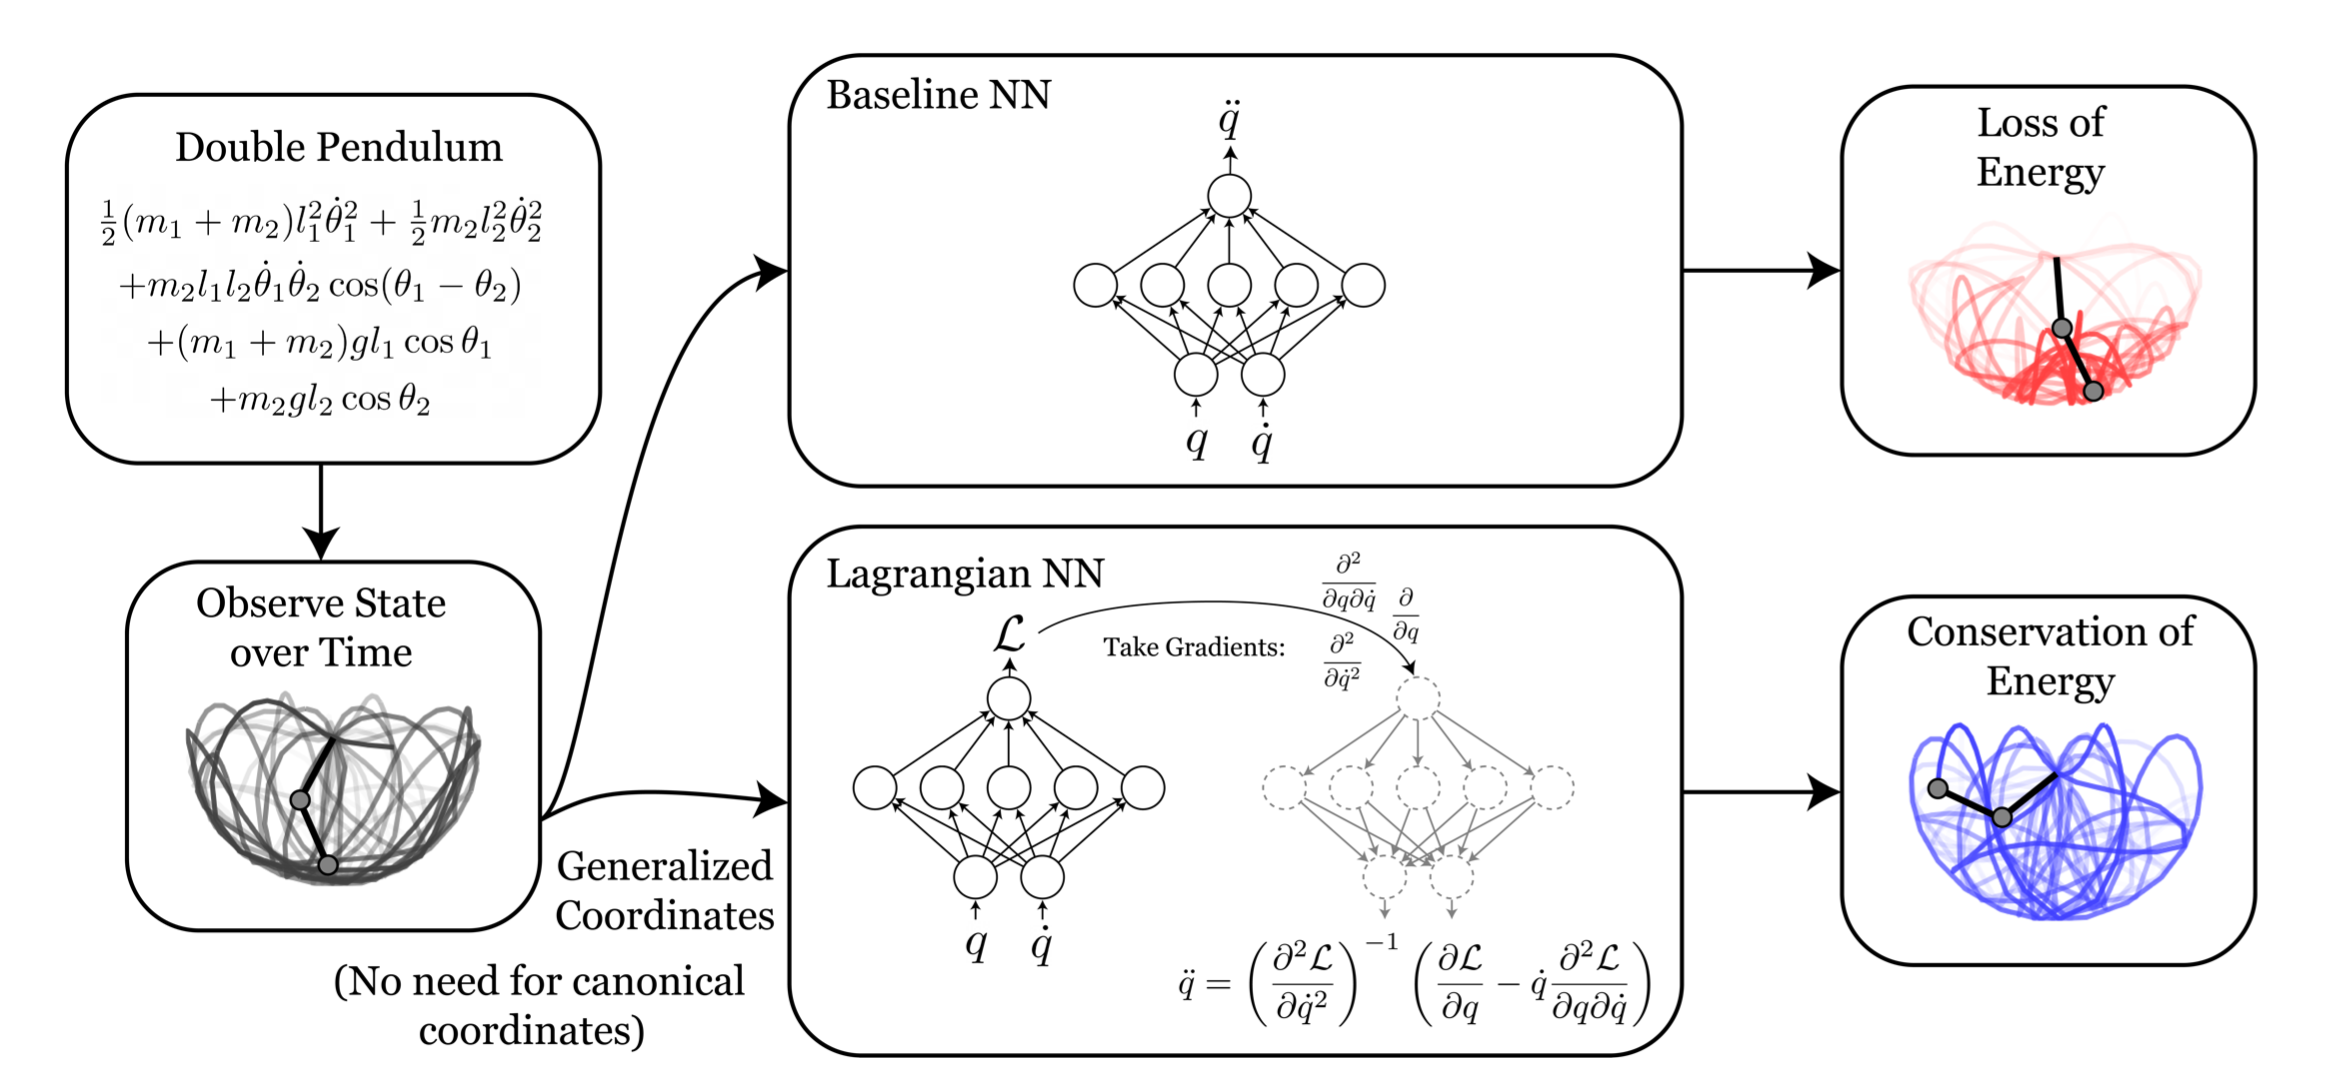
\includegraphics[width=0.99\textwidth]{lnn.png}
		\caption{Схема работы Lagrangian Neural Networks (LNN) моделирования динамики двойного маятника в сравнении с базовым решением (Baseline NN)}
	\end{figure}

	
	\subsection{DeLaN}
	Работа, в котором авторы рассматривают моделирование определенных типов лагранжевых систем. Предполагается, что кинетическая энергия является $T = \dot{q}^TM\dot{q}$, где M — q-зависимая положительно определенная матрица. 
	
	Этот подход хорошо работает для динамики твердого тела, которая включает в себя множество систем, встречающихся в робототехнике. Однако многие системы не обладают такой кинетической энергией: заряженная частица в магнитном поле, быстро движущийся объект в СТО.
	
	\subsection{LNN}
	Лагранжевы нейронные сети(LNN)
	
	\textbf{Сравнение}
		\begin{figure}[h]
			\centering
			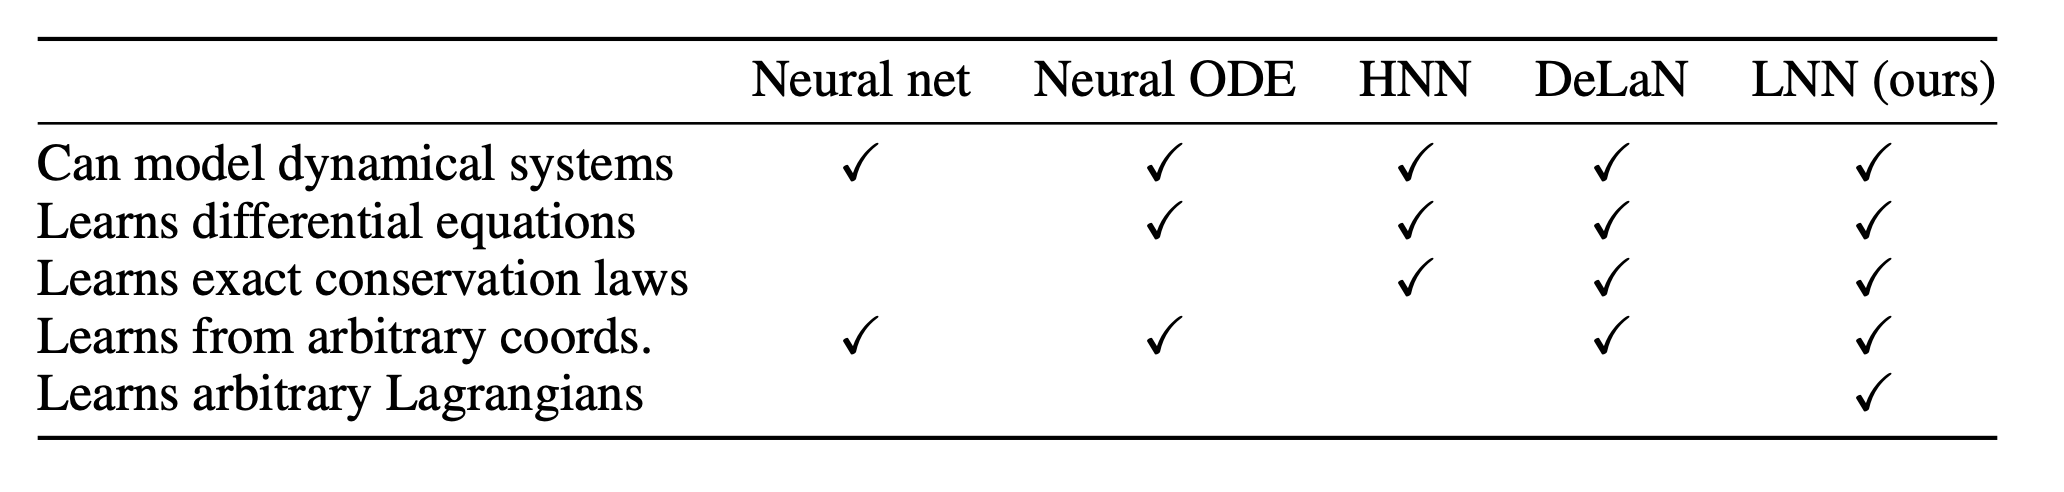
\includegraphics[width=1.05\textwidth]{comparison.png}
			\caption{Сравнение подходов моделирования физических систем нейронными сетями}
		\end{figure}
	
	
	\subsection{Сверточные лагранжевы нейронные сети}
	Добавление сверточных слоев в LNN/DeLaN
	
	\section{Вычислительный эксперимент}
	Целью вычислительного эксперимента является 
	В рамках вычислительного эксперимента написан программный комплекс для решения поставленных задач~\cite{source_code}.
	
	\subsection{Данные}
	


	\section{Заключение}
	В работе рассмотрена задача 
	
	\bibliographystyle{unsrt}
	\bibliography{Severilov2022MasterThesisCite.bib}

	%\bibliographystyle{unsrt}
	%\begin{thebibliography}{99}
		
	
	%	\bibitem{source_code}
%		\textit{Severilov}. Project source code is available at:~\url{https://github.com/severilov/BCI-thesis}, 2021.
	%\end{thebibliography}
	
\end{document}

